\title{CS 613 - Machine Learning}
\author{
        Assignment 2 - Linear Regression\\
        Alex Lapinski\\
        Fall 2016
}
\date{10/20/2016}
\documentclass[12pt]{article}
\usepackage[margin=0.7in]{geometry}
\usepackage{graphicx}
\usepackage{float}
\usepackage{comment}
\usepackage{amsmath}
\graphicspath{{../graphs/}}

\begin{document}
\maketitle

\section{Theory}\label{theory}
\subsection{Standardize Data}\label{standardize data}
$\mu = \frac{-2+-5+-3+0+-8+-2+1+5+-1+6}{10} = \frac{-9}{10} = -0.9\\
\sigma = \sqrt{\frac{(-2+0.9)^2+(-5+0.9)^2+(-3+0.9)^2+(0+0.9)^2+(-8+0.9)^2+(-2+0.9)^2+(1+0.9)^2+5+0.9)^2+(-1+0.9)^2+(6+0.9)^2}{10-1}}\\
\sigma = \sqrt{\frac{(-1.1)^2+(-4.1)^2+(-2.1)^2+(0.9)^2+(-7.1)^2+(-1.1)^2+(1.9)^2+(5.9)^2+(-0.1)^2+(6.9)^2}{9}}\\
\sigma = \sqrt{\frac{1.21+16.81+4.41+0.81+50.41+1.21+3.61+34.81+0.01+47.61}{9}}\\
\sigma = \sqrt{\frac{160.9}{9}} = \sqrt{17.87} = 4.23$\\
\hfill \break

$
 \begin{bmatrix}
	-2 & 1\\
	-5 & -4\\	
	-3 & 1\\
	0 & 3\\
	-8 & 11\\
	-2 & 5\\
	1 & 0\\
	5 & -1\\
	-1 & -3\\
	6 & 1\\
\end{bmatrix}
=
\begin{bmatrix}
	(-2+0.9)/4.23 & 1\\
	(-5+0.9)/4.23 & -4\\	
	(-3+0.9)/4.23 & 1\\
	(0+0.9)/4.23 & 3\\
	(-8+0.9)/4.23 & 11\\
	(-2+0.9)/4.23 & 5\\
	(1+0.9)/4.23 & 0\\
	(5+0.9)/4.23 & -1\\
	(-1+0.9)/4.23 & -3\\
	(6+0.9)/4.23 & 1\\
\end{bmatrix}
=
\begin{bmatrix}
	-0.26 & 1\\
	-0.97 & -4\\	
	-0.50 & 1\\
	 0.21 & 3\\
	-1.68 & 11\\
	-0.26 & 5\\
	0.45 & 0\\
	1.40 & -1\\
	-0.02 & -3\\
	1.63 & 1\\
\end{bmatrix}
$
\subsection{Add Bias}\label{bias}
$
\begin{bmatrix}
	1 & -0.26 & 1\\
	1 & -0.97 & -4\\	
	1 & -0.50 & 1\\
	1 &  0.21 & 3\\
	1 & -1.68 & 11\\
	1 & -0.26 & 5\\
	1 & 0.45 & 0\\
	1 & 1.40 & -1\\
	1 & -0.02 & -3\\
	1 & 1.63 & 1\\
\end{bmatrix}
$
\subsection{Find Theta}\label{theta}
$\theta = (X^TX)^-1X^TY$\\
\hfill \break
$X = 
\begin{bmatrix}
	1 & -0.26\\
	1 & -0.97\\	
	1 & -0.50\\
	1 &  0.21\\
	1 & -1.68\\
	1 & -0.26\\
	1 & 0.45\\
	1 & 1.40\\
	1 & -0.02\\
	1 & 1.63\\
\end{bmatrix}
Y = 
\begin{bmatrix}
	1\\
	-4\\	
	1\\
	3\\
	11\\
	5\\
	0\\
	-1\\
	-3\\
	1\\
\end{bmatrix}
$\\
$
X^TX = \begin{bmatrix}
	1 & 1 & 1 & 1 & 1 & 1 & 1 & 1 & 1 & 1\\
	-0.26 & -0.97 & -0.50 & 0.21 & -1.68 & -0.26 & 0.45 & 1.40 & -0.02 & 1.63\\
\end{bmatrix}
\begin{bmatrix}
	1 & -0.26\\
	1 & -0.97\\	
	1 & -0.50\\
	1 &  0.21\\
	1 & -1.68\\
	1 & -0.26\\
	1 & 0.45\\
	1 & 1.40\\
	1 & -0.02\\
	1 & 1.63\\
\end{bmatrix}\\
$
$
X^TX = 
\begin{bmatrix}
 10 & 0.00\\
0.00 & 9.01\\
\end{bmatrix}\\
\hfill \break
\hfill \break
(X^TX)^-1 = \frac{1}{|X^TX|}\begin{bmatrix}9.01 & 0\\ 0 & 10\end{bmatrix} = \frac{1}{10*9.01 - 0}\begin{bmatrix}9.01 & 0\\ 0 & 10\end{bmatrix}=\begin{bmatrix}9.01/90.1 & 0\\ 0 & 10/90.1\end{bmatrix} = \begin{bmatrix}0.01 & 0\\ 0 & 0.11\end{bmatrix}\\
\hfill \break
\hfill \break
(X^TX)^-1X = \begin{bmatrix}0.01 & 0.00\\ 0.00 & 0.11\\\end{bmatrix}
\begin{bmatrix}
	1 & 1 & 1 & 1 & 1 & 1 & 1 & 1 & 1 & 1\\
	-0.26 & -0.97 & -0.50 & 0.21 & -1.68 & -0.26 & 0.45 & 1.40 & -0.02 & 1.63\\
\end{bmatrix}\\
\hfill \break
\hfill \break
(X^TX)^-1X^T = \begin{bmatrix}
	0.1 & 0.1 & 0.1 & 0.1 & 0.1 & 0.1 & 0.1 & 0.1 & 0.1 & 0.1\\
	-0.03 & -0.11 & -0.06 & 0.02 & -0.19 & -0.03 & 0.05 & 0.16 & 0 & 0.18\\
\end{bmatrix}\\
\hfill \break
\hfill \break
(X^TX)^-1X^TY = 
\begin{bmatrix}
	0.1 & 0.1 & 0.1 & 0.1 & 0.1 & 0.1 & 0.1 & 0.1 & 0.1 & 0.1\\
	-0.03 & -0.11 & -0.06 & 0.02 & -0.19 & -0.03 & 0.05 & 0.16 & 0 & 0.18\\
\end{bmatrix}
\begin{bmatrix}
	1\\
	-4\\	
	1\\
	3\\
	11\\
	5\\
	0\\
	-1\\
	-3\\
	1\\
\end{bmatrix}
= 
\begin{bmatrix}	1.4 & -1.75 \\\end{bmatrix}
\\
\hfill \break
\hfill \break
\theta = \begin{bmatrix}	1.4 & -1.75 \\\end{bmatrix}
$

\newpage
\section{Closed Form Linear Regression}\label{linreg}

\begin{enumerate}
\item Final Model: $y=3343.27586207+1036.63016523x_{:,1} - 295.66859639x_{:,2}$
\item Root Mean Squared Error: $653.76012597$
\end{enumerate}

\section{S-Folds Cross-Validation}\label{linreg}

\begin{enumerate}
\item With S = 5 (as required), RMSE = 636.315054765
\item With S = 6 (to test other values), RMSE = 621.823391267
\item With S = 7 (to test other values), RMSE = 640.86061133
\end{enumerate}

\section{Locally-Weighted Linear Regression}
\begin{enumerate}
\item With k = 1 (as required), RMSE = 242.531418672
\item With k = 2 (to test other values), RMSE = 435.493965086
\item With k = 0.5 (to test other values), RMSE = 216.575016394
\item With k = 0.75 (to test other values), RMSE = 209.853739868
\end{enumerate}


\newpage
\section{Gradient Descent}

\textbf{Results when $\alpha=0.01$}
\begin{itemize}
\item Final model: $y = 3343.27574946 + 1036.63010327x_{:,1} + -295.66858438x_{:,2}$
\item After 1712 iterations
\item RMSE = 653.760066367
\end{itemize}

\begin{figure}[H]
\begin{center}
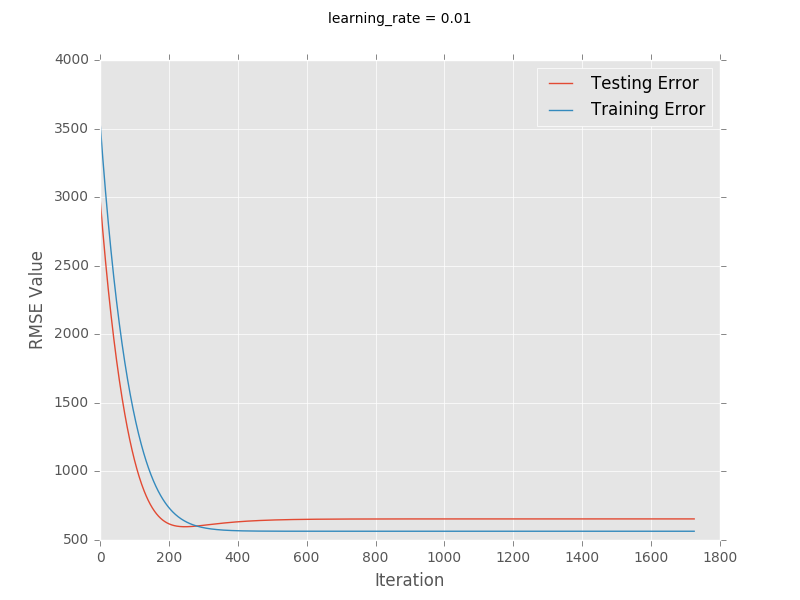
\includegraphics{gradient_descent_errors.png}
\caption{Gradient Descent Progress}
\label{GD}
\end{center}
\end{figure}

\textbf{Results when $\alpha=0.1$}
\begin{itemize}
\item Final model: $y = 3343.27584461 + 1036.63015469x_{:,1} + -295.66859449_{:,2}$
\item After 181 iterations
\item RMSE = 653.760097303
\end{itemize}

\end{document}